This document forms the reference manual for the Burn In Unit based on the Texas Instruments F2802x.

This system has been implemented using several Texas Instruments libraries; digital power v3.\-1, S\-Gen V1.\-01, I\-Q\-Math v1.\-5c and S\-Q\-Math. Please refer to the T\-I documentation pertaining to those libraries and to the C28x device to understand their operation.

This system also uses the System for Standard Commands for Programmable Instruments for C28x, again, refer to the documentation pertaining to that system to understand its use.

\paragraph*{General Operation}

This system operates using the concept of a state machine with multiplexed threading. This allows important tasks, such as signal generation and the monitoring of critical parameters to take precedence while still allowing other less critical tasks to run with acceptable frequency. This is allowed by creating several threads D\-P\-L, A, B and C and iterating them at different interval periods, such that every time the thread is iterated the next single task in that thread is run.

\subparagraph*{Fast (D\-P\-L) Thread}

The D\-P\-L thread is the fastest thread, is coded in assembly and consists of only two tasks. It is the only thread that uses an interrupt to iterate. Thus the tasks are formed by an interrupt service routine (I\-S\-R). This allows the D\-P\-L thread to interrupt the ongoing action of any of the other threads. This means that as long as the length of time each of the tasks take to execute is less than the interval time, then the threads operation will be deterministic. It is within this thread's two tasks that the critical and time-\/sensitive actions of the program are carried out. The thread I\-S\-R is triggered by a start of conversion (S\-O\-C) signal from the master enhanced pulse width modulation (e\-P\-W\-M) peripheral. This occurs at a frequency of 33 k\-Hz. As there are two tasks on the thread, the frequency of each task is 16.\-5 k\-Hz resulting in a period of 60us.

\subparagraph*{Sequential Iteration Threads}

The remaining threads (A, B, C) iterate by checking the rollover state of different C\-P\-U timers. Their operation and iteration is sequential and so less deterministic. The outline of the handling sequential iteration threads by the state machine is illustrated by the following flow diagram, where N and n rollover to A and 0, respectively whenever they reach their maximum value.


\begin{DoxyImage}
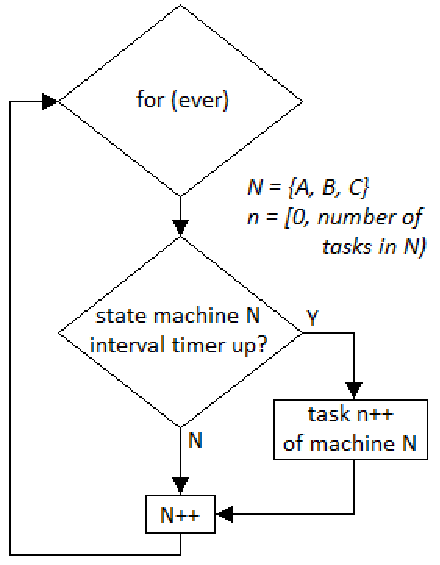
\includegraphics[width=5cm]{state_machine_loop}
\caption{Sequential iteration thread state machine}
\end{DoxyImage}


The frequency of tasks can be determined from the period of the interval timers using the following equation, where {\itshape n} is the number of tasks in the thread and {\itshape T$_{\mbox{in}}$ } is the interval timer period. \[ f_{ta}= \frac{1}{T_{in} \times n} \] With interval periods such that {\itshape T$_{\mbox{A}}$ } {\ttfamily $<$} {\itshape T$_{\mbox{B}}$ } {\ttfamily $<$} {\itshape T$_{\mbox{A}}$ } this results in the flow of execution illustrated by the following figure.


\begin{DoxyImage}
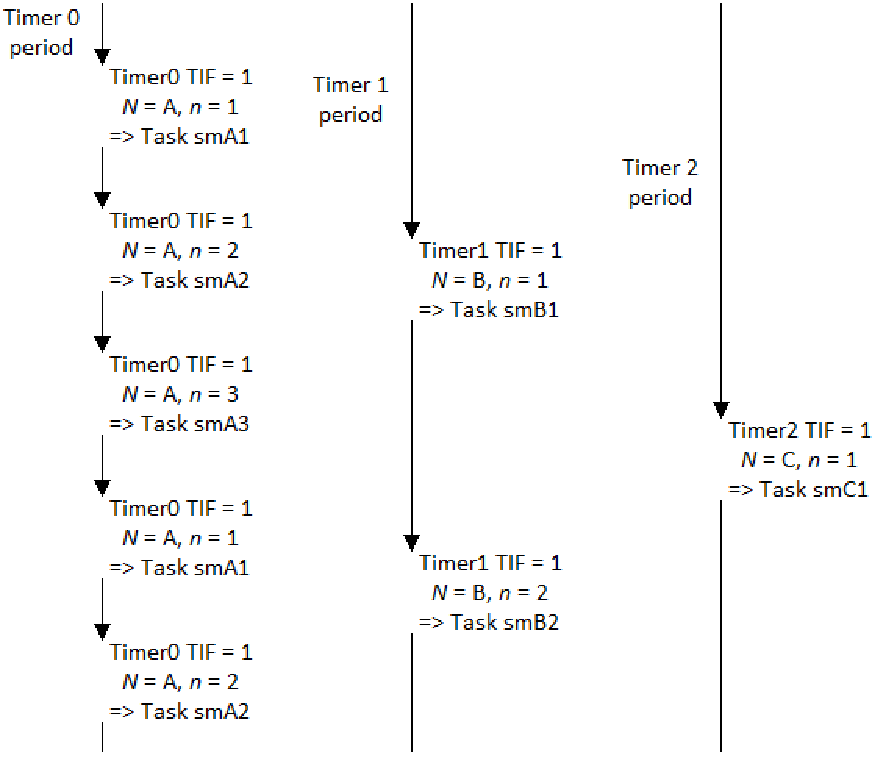
\includegraphics[width=8cm]{seq_state_machine_task_itr}
\caption{Sequence of thread tasks}
\end{DoxyImage}


\paragraph*{Digital Power Control}

The control of the power, voltage and current is managed using control loop logic, normally one loop for each stage (Transformer, A\-C, each of the four loads). These control loops are formed from a set of macros and helper functions.

Each of these macros acts as a block of functionality, much like a black-\/box electronic component, allowing their terminals to be wired together in the required order with nets. Once initialised and configured, or connected, correctly the macro blocks are executed, sequentially, by calling the appropriate code from an assembly I\-S\-R. In this case, this is what forms the D\-P\-L I\-S\-R tasks. Each block performs a precisely defined computation and delivers the result to the appropriate net-\/list variables. Each control loop's net vairables and operation parameter variables are grouped together and stored in a structure (\hyperlink{structchannel_parameters}{channel\-Parameters}), with one such structure for each control loop.

The basic use of macros that are available within the program can be broken down into three parts\-:
\begin{DoxyEnumerate}
\item Initialisation\-: the macro blocks are initialised from the program by using a C callable function, D\-P\-L\-\_\-\-Init(), which is contained within the assembly file D\-P\-L\-\_\-\-I\-S\-R.\-asm.
\item Configuration\-: C pointers of the macro block terminals are assigned to net nodes to form the desired control structure, i.\-e., the control loop.
\item Execution\-: Macro block code is executed in the assembly I\-S\-R, \hyperlink{_pwm_8h_a5532a53363218854b0e4b15049d773f7}{D\-P\-L\-\_\-\-I\-S\-R()}.
\end{DoxyEnumerate}

\subparagraph*{Boost Load Control}

The following figure shows a diagram that illustrates the macro and net view of the control loop for one of the load boost converter stages. The loop depicted is current controlled. It uses a macro to retrieve a reading from an A\-D\-C peripheral to obtain a value that indicates the level of the current at the low side of the load input, C\-H\-A\-Nn I$_{\mbox{S\-N\-S}}$ . This value is used as the feedback into a 2-\/pole 2-\/zero filter macro where it is compared to the user-\/set reference value and the output value is varied up or down, using the filter coefficients, as needed to move it towards matching the reference. This output value is then used by another macro to set the duty of the e\-P\-W\-M peripheral that controls the switching of the converter, C\-H\-A\-Nn P\-W\-M.

Another macro retrieves a value from a second A\-D\-C that represents the voltage level across the load input, C\-H\-A\-Nn V$_{\mbox{S\-N\-S}}$ . A task in one of the sequential iteration threads compares this value to the user-\/set allowable voltage limit, the O\-V\-P limit. If the value is above this limit the control loop output is disabled and an over-\/current protection alert is raised.


\begin{DoxyImage}
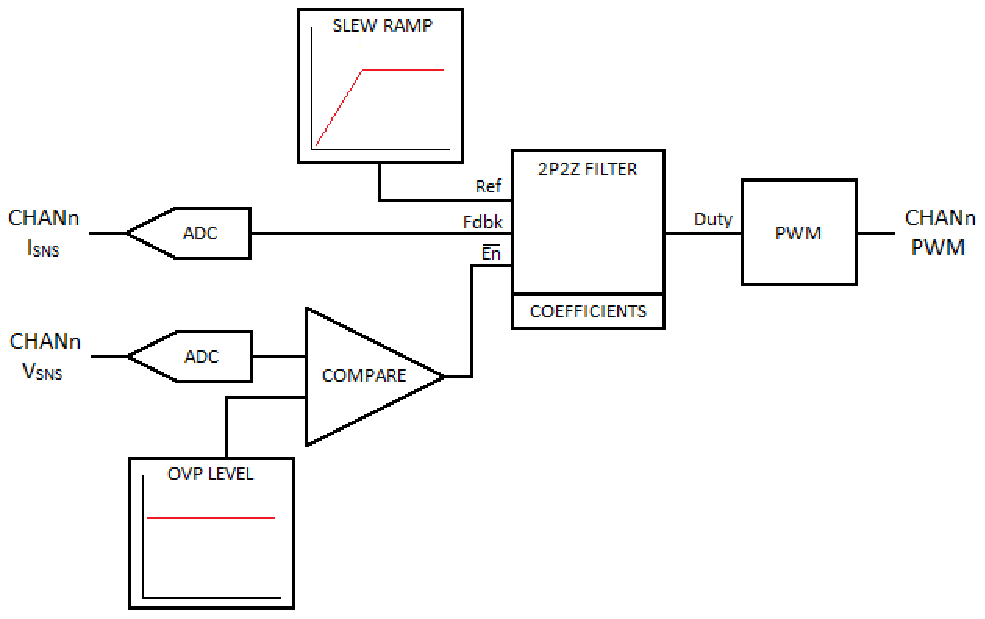
\includegraphics[width=10cm]{boost_load_loop}
\caption{Macro view of control loop for single boost load}
\end{DoxyImage}


\subparagraph*{Inter-\/\-Boost Control}

The following figure shows a diagram that illustrates the macro and net view of the control loop for the inter-\/boost, or \char`\"{}middle\char`\"{}, boost converter stage. The loop depicted is voltage controlled. It uses a macro to retrieve a reading from an A\-D\-C peripheral to obtain a value that indicates the level of the voltage across the stage output, D\-C H\-V V$_{\mbox{S\-N\-S}}$ . This value is used as the feedback into a 3-\/pole 3-\/zero filter macro where it is compared to the user-\/set reference value and the output value is varied up or down, using the filter coefficents, as needed to move towards matching the reference. This output value is then used by another macro to set the duty of the e\-P\-W\-M peripheral that controls the switching of the converter, I\-N\-T\-B\-S\-T P\-W\-M.

Another macro retrieves a value from a second A\-D\-C that represents the current level at the low side of the input, D\-C M\-I\-D I$_{\mbox{S\-N\-S}}$ . An on-\/board analogue comparator compares this value against the user-\/set allowable current limit, the O\-C\-P limit. If the value is above this limit the comparator output sets the related trip-\/zone, quickly disabling the control loop output in software and hardware, H\-V E\-N.


\begin{DoxyImage}
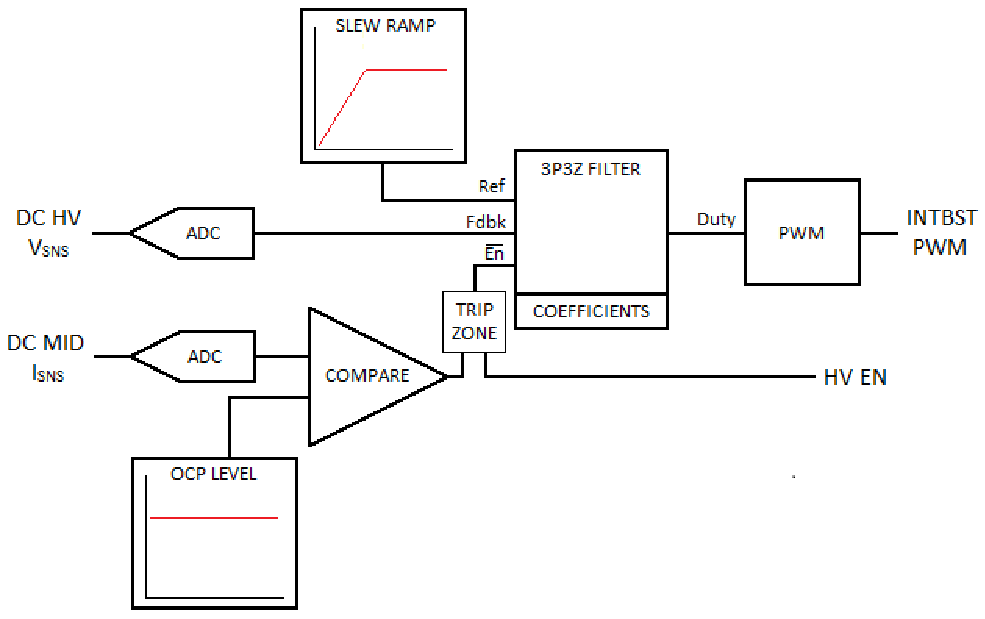
\includegraphics[width=10cm]{boost_xfmr_loop}
\caption{Macro view of control loop for inter-\/boost}
\end{DoxyImage}


\subparagraph*{A\-C Bridge Control}

The following figure shows a diagram that illustrates he macro and a net view of the control loop for the A\-C bridge converter stage. The loop depicted is both voltage {\itshape and} current controlled. It uses a macro to retrieve a reading from an A\-D\-C peripheral to obtain a value that indicates the voltage level across the stage output, A\-C V$_{\mbox{S\-N\-S}}$ . This value is used as the feedback into a 3-\/pole 3-\/zero filter macro where it is compared to the generated sine wave reference and the output value is varied up or down, using the filter coefficients, as needed to move towards matching the reference.

Another macro retrieves a value from a second A\-D\-C that represents the current level at the low side of the stage input, A\-C I$_{\mbox{S\-N\-S}}$ . This value is used as the feedback into a 2-\/pole 2-\/zero filter macro where it is compared to the output of the 3-\/pole 3-\/zero filter macro and the output is varied up or down, using the filter coefficents, as needed to move towards matching the reference.

An on board analogue comparator also compares this A\-C I$_{\mbox{S\-N\-S}}$  vlaueagainst the user-\/set allowable current limit, the O\-C\-P limit. If the value is above the limit tha comparator output sets the relted trip zone, quickly disabling the control loop output and all other stages output, S\-T\-O\-P A\-L\-L.


\begin{DoxyImage}
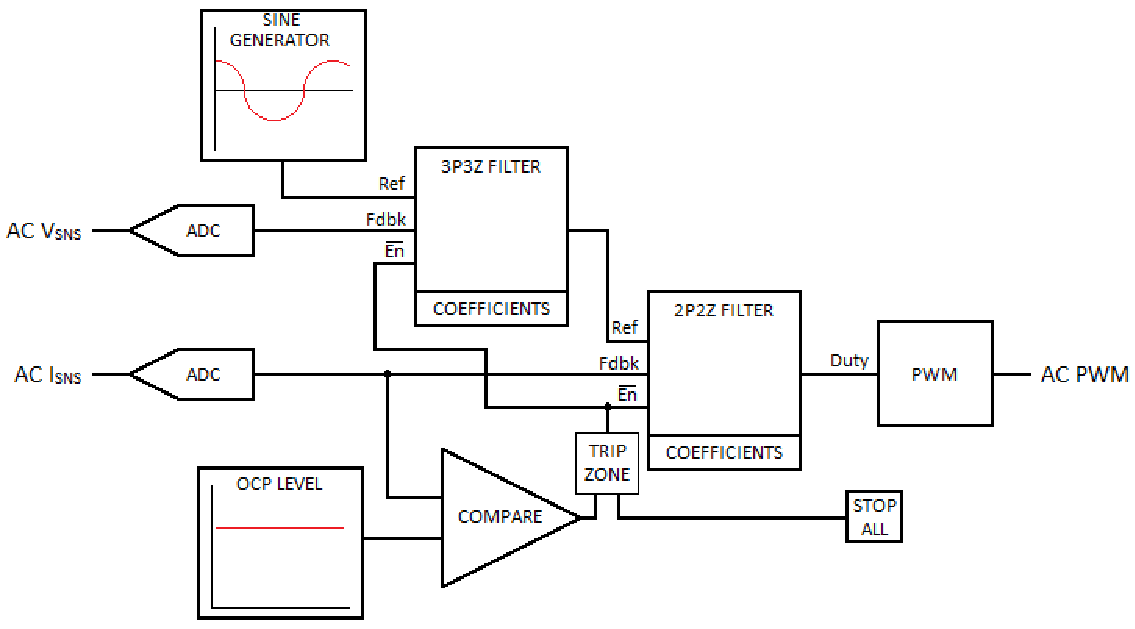
\includegraphics[width=10cm]{ac_bridge_loop}
\caption{Macro view of control loop for A\-C bridge}
\end{DoxyImage}
 